
\documentclass[aspectratio=169]{beamer}

%\usepackage[table]{xcolor}
\mode<presentation> {
\setbeamercovered{transparent}
  \usetheme{Boadilla}

%  \usetheme{Pittsburgh}
%\usefonttheme[2]{sans}
\renewcommand{\familydefault}{cmss}
%\usepackage{lmodern}
%\usepackage[T1]{fontenc}
%\usepackage{palatino}
%\usepackage{cmbright}
\usepackage{bm}
\usepackage{stackrel}
\usepackage{array}
\usepackage{listings}
\useinnertheme{rectangles}
}
\usepackage{amsmath}
\setbeamercolor{normal text}{fg=black}
\setbeamercolor{structure}{fg= blue}
\definecolor{trial}{cmyk}{1,0,0, 0}
\definecolor{trial2}{cmyk}{0.00,0,1, 0}
\definecolor{darkgreen}{rgb}{0,.4, 0.1}
\usepackage{array}
\beamertemplatesolidbackgroundcolor{white}  \setbeamercolor{alerted
text}{fg=red}
\usepackage{tcolorbox}
\setbeamertemplate{caption}[numbered]\newcounter{mylastframe}

\font\domino=domino
\def\die#1{{\domino#1}}
\usepackage{tikz}
\usetikzlibrary{calc}
\usetikzlibrary{arrows}
\usepackage{colortbl}

\renewcommand{\familydefault}{cmss}
%\usepackage[all]{xy}

\usepackage{tikz}
\usepackage{lipsum}
\usepackage{pgfplots}
\pgfplotsset{compat=1.17}
\usepackage{booktabs}

\lstset{%
  language=R,
  basicstyle=\ttfamily\small,
  keywordstyle=\color{blue},
  commentstyle=\color{darkgreen},
  stringstyle=\color{red},
  showstringspaces=false,
  breaklines=true,
  frame=single,
  backgroundcolor=\color{gray!10}
}

 \newenvironment{changemargin}[3]{%
 \begin{list}{}{%
 \setlength{\topsep}{0pt}%
 \setlength{\leftmargin}{#1}%
 \setlength{\rightmargin}{#2}%
 \setlength{\topmargin}{#3}%
 \setlength{\listparindent}{\parindent}%
 \setlength{\itemindent}{\parindent}%
 \setlength{\parsep}{\parskip}%
 }%
\item[]}{\end{list}}
\usetikzlibrary{arrows}

\usecolortheme{lily}

\newtheorem{com}{Comment}
\newtheorem{lem} {Lemma}
\newtheorem{prop}{Proposition}
\newtheorem{condition}{Condition}
\newtheorem{thm}{Theorem}
\newtheorem{defn}{Definition}
\newtheorem{cor}{Corollary}
\newtheorem{obs}{Observation}
 \numberwithin{equation}{section}

\makeatletter
\def\beamerorig@set@color{%
  \pdfliteral{\current@color}%
  \aftergroup\reset@color
}
\def\beamerorig@reset@color{\pdfliteral{\current@color}}
\makeatother
\setbeamertemplate{navigation symbols}{}

\useoutertheme{miniframes}
\title[PLSC 30700]{Linear Models Lecture 9: Probit}

\author{Robert Gulotty}
\institute[Chicago]{University of Chicago}
\vspace{0.3in}

\pgfmathdeclarefunction{normalpdf}{3}{%
  \pgfmathparse{1/(#3*sqrt(2*pi))*exp(-((#1)-(#2))^2/(2*(#3)^2))}%
}
\begin{document}

\begin{frame}
\maketitle
\end{frame}

%%%%%%%%%%%%%%%%%%%%%%%%%%%%%%%%%%%%%%%%%%%%%%%%%%%%%%%%%%%%
\section{Binary Outcomes and the Linear Probability Model}
%%%%%%%%%%%%%%%%%%%%%%%%%%%%%%%%%%%%%%%%%%%%%%%%%%%%%%%%%%%%

\begin{frame}{Binary Outcomes and the BLP}

Recall from Lecture 2, the \textbf{best linear predictor} (BLP):
\[
\beta = \arg\min_b \, \mathbb{E}\left[(Y - X'b)^2\right]
\]

\pause

\textbf{What happens when $Y \in \{0,1\}$?}

\pause

The conditional expectation function is now a probability:
\[
m(x) = \mathbb{E}[Y \mid X = x] = P(Y = 1 \mid X = x)
\]

\pause

The BLP still exists --- OLS estimates $\beta$ by solving the same normal equations:
\[
\sum_{i=1}^n X_i(Y_i - X_i'\hat\beta) = 0
\]

This is the \textbf{linear probability model} (LPM).

\end{frame}

%%%%%%%%%%%%%%%%%%%%%%%%%%%%%%%%%%%%%%%%%%%%%%%%%%%%%%%%%%%%

\begin{frame}{LPM: Consistent for Average Marginal Effects}

Even if the true CEF $P(Y=1 \mid X)$ is nonlinear, OLS estimates a useful object.

\pause

Recall the BLP--CEF distinction from Lecture 2:
\begin{itemize}
    \item The BLP $X'\beta$ need not equal the CEF $m(x)$
    \item But $\beta$ is consistent for the \textbf{average marginal effect} under mild conditions
\end{itemize}

\pause

\textbf{Built-in heteroskedasticity} (recall Lecture 6):

If $Y_i \in \{0,1\}$, then
\[
\operatorname{Var}(Y_i \mid X_i) = p(X_i)(1 - p(X_i))
\]
where $p(X_i) = P(Y_i = 1 \mid X_i)$.

\pause

The variance depends on $X_i$ by construction. The LPM \textbf{always} requires heteroskedasticity-robust standard errors (HC2).

\end{frame}

%%%%%%%%%%%%%%%%%%%%%%%%%%%%%%%%%%%%%%%%%%%%%%%%%%%%%%%%%%%%

\begin{frame}{Limitations of the Linear Probability Model}

\begin{columns}
\begin{column}{0.48\textwidth}

\textbf{Problems:}
\begin{itemize}
    \item Predictions outside $[0,1]$
    \item Poor approximation in tails
    \item Marginal effects constant (may be unrealistic)
\end{itemize}

\pause

\textbf{Motivation:} A model that respects the $[0,1]$ constraint.

\pause

\textbf{Single-index model:}
\[
P(Y = 1 \mid X) = G(X'\beta)
\]
where $G: \mathbb{R} \to [0,1]$ is a known link function.

\end{column}
\begin{column}{0.48\textwidth}

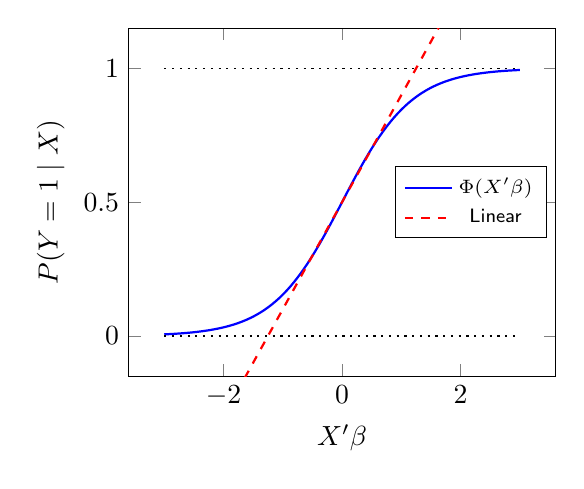
\begin{tikzpicture}
\begin{axis}[
  width=7cm, height=6cm,
  domain=-3:3, samples=100,
  xlabel={$X'\beta$}, ylabel={$P(Y=1 \mid X)$},
  ymin=-0.15, ymax=1.15,
  legend style={at={(0.98,0.5)}, anchor=east, font=\scriptsize},
  every axis plot/.append style={thick}
]
\addplot[blue] {1/(1+exp(-1.7*x))};
\addlegendentry{$\Phi(X'\beta)$}
\addplot[red, dashed] {0.5 + 0.4*x};
\addlegendentry{Linear}
\addplot[black, dotted, thin] coordinates {(-3,0)(3,0)};
\addplot[black, dotted, thin] coordinates {(-3,1)(3,1)};
\end{axis}
\end{tikzpicture}

\end{column}
\end{columns}

\end{frame}

%%%%%%%%%%%%%%%%%%%%%%%%%%%%%%%%%%%%%%%%%%%%%%%%%%%%%%%%%%%%

\begin{frame}{From LPM to Probit}

\textbf{Two common link functions:}

\medskip

\begin{tabular}{lll}
\textbf{Probit:} & $G = \Phi$ & (standard normal CDF) \\
\textbf{Logit:} & $G = \Lambda$ & (logistic CDF: $e^x/(1+e^x)$)
\end{tabular}

\pause

\bigskip

Both map $\mathbb{R} \to (0,1)$, are symmetric about $1/2$, and produce nearly identical fitted values.

\pause

\bigskip

\textbf{Why Probit?}
\begin{itemize}
    \item Natural latent variable interpretation ($\varepsilon \sim N(0,1)$)
    \item Connects to the normal distribution theory from Lectures 1 and 7
    \item Extends naturally to measurement models (IRT, later today)
\end{itemize}

\end{frame}

%%%%%%%%%%%%%%%%%%%%%%%%%%%%%%%%%%%%%%%%%%%%%%%%%%%%%%%%%%%%
\section{The Probit Model}
%%%%%%%%%%%%%%%%%%%%%%%%%%%%%%%%%%%%%%%%%%%%%%%%%%%%%%%%%%%%

\begin{frame}{Latent Variable Representation}

Suppose there exists an unobserved variable:

\[
Y_i^* = X_i'\beta + \varepsilon_i
\]

\pause

Observed outcome:

\[
Y_i = \mathbf{1}\{Y_i^* > 0\}
\]

\pause

Assume:

\[
\varepsilon_i \sim N(0,1)
\]

\pause

Then:

\[
P(Y_i=1 \mid X_i)
=
P(\varepsilon_i > -X_i'\beta)
=
\Phi(X_i'\beta)
\]

\pause

This is the \textbf{Probit model}.
\end{frame}

%%%%%%%%%%%%%%%%%%%%%%%%%%%%%%%%%%%%%%%%%%%%%%%%%%%%%%%%%%%%

\begin{frame}{Identification and Scale Normalization}

In the latent model:

\[
Y_i^* = X_i'\beta + \varepsilon_i, \qquad \varepsilon_i \sim N(0,\sigma^2)
\]

\pause

Then:

\[
P(Y_i=1 \mid X_i)
=
\Phi\left(\frac{X_i'\beta}{\sigma}\right)
\]

\pause

Only $\beta/\sigma$ is identified --- the data cannot distinguish $(\beta, \sigma)$ from $(c\beta, c\sigma)$.

\pause

\textbf{Normalization:} Set $\operatorname{Var}(\varepsilon_i) = 1$.

\pause

\begin{tcolorbox}[colback=blue!5, colframe=blue!50, title=Key Point]
Probit coefficients are identified only up to scale. We cannot interpret $\beta_j$ the same way as in OLS. This is fundamentally different from the linear model.
\end{tcolorbox}

\end{frame}

%%%%%%%%%%%%%%%%%%%%%%%%%%%%%%%%%%%%%%%%%%%%%%%%%%%%%%%%%%%%

\begin{frame}{Marginal Effects}

In the linear model: $\partial \mathbb{E}[Y \mid X]/\partial x_j = \beta_j$.

\pause

In the Probit model:
\[
\frac{\partial P(Y=1 \mid X)}{\partial x_j}
=
\phi(X'\beta) \cdot \beta_j
\]

\pause

The marginal effect \textbf{depends on $X$} through $\phi(X'\beta)$.

\pause

\bigskip

\textbf{Average Marginal Effect} (AME):
\[
\widehat{\text{AME}}_j = \frac{1}{n}\sum_{i=1}^n \phi(X_i'\hat\beta)\,\hat\beta_j
\]

\pause

\begin{itemize}
    \item The AME averages over the observed distribution of $X$
    \item This is the natural analog of the OLS coefficient for binary outcomes
    \item Computing the AME requires the \textbf{delta method} (Lecture 10) for standard errors
\end{itemize}

\end{frame}

%%%%%%%%%%%%%%%%%%%%%%%%%%%%%%%%%%%%%%%%%%%%%%%%%%%%%%%%%%%%

\begin{frame}{Marginal Effects: Graphical Intuition}

\begin{center}
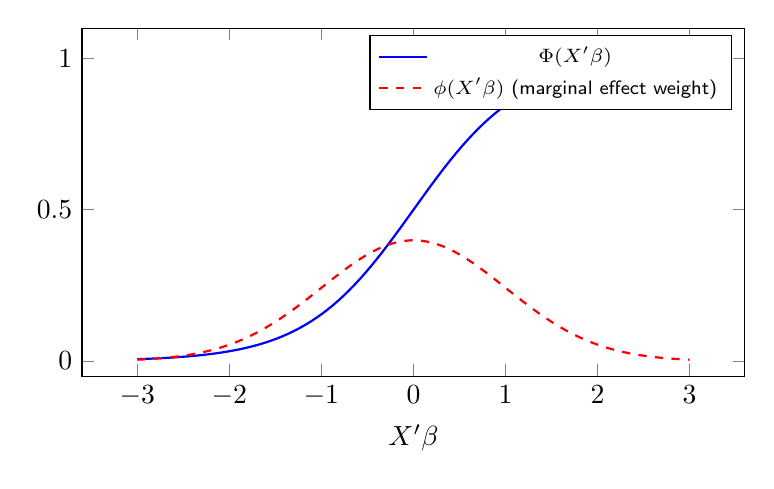
\begin{tikzpicture}
\begin{axis}[
  width=10cm, height=6cm,
  domain=-3:3, samples=100,
  xlabel={$X'\beta$}, ylabel={},
  ymin=-0.05, ymax=1.1,
  legend style={at={(0.98,0.98)}, anchor=north east, font=\scriptsize},
  every axis plot/.append style={thick}
]
% CDF (logistic approx to Phi)
\addplot[blue] {1/(1+exp(-1.7*x))};
\addlegendentry{$\Phi(X'\beta)$}
% PDF (standard normal)
\addplot[red, dashed] {exp(-x^2/2)/sqrt(2*pi)};
\addlegendentry{$\phi(X'\beta)$ (marginal effect weight)}
\end{axis}
\end{tikzpicture}
\end{center}

\pause

Marginal effects are largest near $X'\beta = 0$ (where the CDF is steepest) and vanish in the tails.

\end{frame}

%%%%%%%%%%%%%%%%%%%%%%%%%%%%%%%%%%%%%%%%%%%%%%%%%%%%%%%%%%%%
\section{Maximum Likelihood Estimation}
%%%%%%%%%%%%%%%%%%%%%%%%%%%%%%%%%%%%%%%%%%%%%%%%%%%%%%%%%%%%

\begin{frame}{Likelihood for the Probit Model}

Recall from Lecture 7: we developed the general MLE framework under normality. Now we apply it to a \textbf{nonlinear} model.

\pause

\bigskip

Assuming conditional independence, the likelihood is:

\[
L_n(\beta)
=
\prod_{i=1}^n
\Phi(X_i'\beta)^{Y_i}
\left(1-\Phi(X_i'\beta)\right)^{1-Y_i}
\]

\pause

Log-likelihood:

\[
\ell_n(\beta)
=
\sum_{i=1}^n
\left[
Y_i \log \Phi(X_i'\beta)
+
(1-Y_i)\log\left(1-\Phi(X_i'\beta)\right)
\right]
\]

\pause

We estimate $\hat\beta_{\text{MLE}} = \arg\max_\beta \, \ell_n(\beta)$.

\end{frame}

%%%%%%%%%%%%%%%%%%%%%%%%%%%%%%%%%%%%%%%%%%%%%%%%%%%%%%%%%%%%

\begin{frame}{Score Function}

Let $\phi(\cdot)$ denote the standard normal pdf, $\Phi(\cdot)$ the CDF.

\pause

The individual score contribution:

\[
s_i(\beta) = \frac{\partial \ell_i}{\partial \beta}
=
\frac{\phi(X_i'\beta)}{\Phi(X_i'\beta)(1-\Phi(X_i'\beta))}
\left(Y_i - \Phi(X_i'\beta)\right) X_i
\]

\pause

The total score:

\[
S_n(\beta) = \sum_{i=1}^n s_i(\beta) = \sum_{i=1}^n w_i \left(Y_i - \Phi(X_i'\beta)\right) X_i
\]

where $w_i = \phi(X_i'\beta)/[\Phi(X_i'\beta)(1-\Phi(X_i'\beta))]$.

\pause

\bigskip

Setting $S_n(\hat\beta) = 0$ defines the MLE. This is a \textbf{nonlinear} system --- no closed-form solution.

\end{frame}

%%%%%%%%%%%%%%%%%%%%%%%%%%%%%%%%%%%%%%%%%%%%%%%%%%%%%%%%%%%%

\begin{frame}{Score as Moment Condition}

\textbf{Key insight:} Under correct specification, $\mathbb{E}[s_i(\beta_0)] = 0$.

\pause

\bigskip

Compare three estimating equations side by side:

\medskip

\renewcommand{\arraystretch}{1.8}
\begin{tabular}{lll}
\toprule
\textbf{Model} & \textbf{Estimating Equation} & \textbf{Weights} \\
\midrule
OLS & $\displaystyle\sum_i X_i(Y_i - X_i'\beta) = 0$ & Equal \\[6pt]
Probit MLE & $\displaystyle\sum_i w_i(Y_i - \Phi(X_i'\beta))\, X_i = 0$ & $w_i = \frac{\phi}{\Phi(1-\Phi)}$ \\[6pt]
General & $\displaystyle\sum_i g_i(\theta) = 0$ & $\to$ GMM \\
\bottomrule
\end{tabular}
\renewcommand{\arraystretch}{1.0}

\pause

\bigskip

All three are \textbf{sample moment conditions}. GMM (coming later) is the general framework: find $\theta$ such that $\frac{1}{n}\sum_i g(W_i, \theta) = 0$.

\end{frame}

%%%%%%%%%%%%%%%%%%%%%%%%%%%%%%%%%%%%%%%%%%%%%%%%%%%%%%%%%%%%

\begin{frame}{Iterative Estimation: Newton--Raphson}

Unlike OLS, the Probit MLE has no closed-form solution.

\pause

\textbf{Newton--Raphson} iterates:
\[
\beta^{(t+1)} = \beta^{(t)} - \left[H_n(\beta^{(t)})\right]^{-1} S_n(\beta^{(t)})
\]

where $H_n(\beta) = \partial S_n / \partial \beta' = \partial^2 \ell_n / \partial \beta \partial \beta'$ is the Hessian.

\pause

\bigskip

\textbf{Algorithm:}
\begin{enumerate}
    \item Start with an initial guess $\beta^{(0)}$ (e.g., OLS estimates)
    \item Compute score $S_n(\beta^{(t)})$ and Hessian $H_n(\beta^{(t)})$
    \item Update: $\beta^{(t+1)} = \beta^{(t)} - H_n^{-1} S_n$
    \item Repeat until convergence: $\|\beta^{(t+1)} - \beta^{(t)}\| < \varepsilon$
\end{enumerate}

\pause

In practice, \texttt{glm()} in R handles this automatically via Fisher scoring (a variant of Newton--Raphson).

\end{frame}

%%%%%%%%%%%%%%%%%%%%%%%%%%%%%%%%%%%%%%%%%%%%%%%%%%%%%%%%%%%%

\begin{frame}{Why Not Just Use OLS?}

\begin{center}
\renewcommand{\arraystretch}{1.4}
\begin{tabular}{lcc}
\toprule
& \textbf{LPM (OLS)} & \textbf{Probit (MLE)} \\
\midrule
Closed-form solution & Yes & No \\
Predictions in $[0,1]$ & Not guaranteed & Yes \\
Consistent for $\beta$ & --- & Yes (if correctly specified) \\
Consistent for AME & Yes (always) & Yes (if correctly specified) \\
Robust to misspecification & Yes (BLP always exists) & Requires sandwich SEs \\
Efficiency & Lower & Higher (if correct) \\
\bottomrule
\end{tabular}
\renewcommand{\arraystretch}{1.0}
\end{center}

\pause

\begin{tcolorbox}[colback=blue!5, colframe=blue!50]
\textbf{Practical guidance:} LPM is a robust baseline. Probit gains efficiency if the model is correct, but misspecification has consequences.
\end{tcolorbox}

\end{frame}

%%%%%%%%%%%%%%%%%%%%%%%%%%%%%%%%%%%%%%%%%%%%%%%%%%%%%%%%%%%%
\section{Asymptotic Distribution}
%%%%%%%%%%%%%%%%%%%%%%%%%%%%%%%%%%%%%%%%%%%%%%%%%%%%%%%%%%%%

\begin{frame}{Fisher Information for Probit}

The Fisher information matrix is:
\[
\mathcal{I}(\beta)
=
\mathbb{E}\left[\frac{\phi(X'\beta)^2}{\Phi(X'\beta)(1-\Phi(X'\beta))} \, XX'\right]
\]

\pause

\textbf{Derivation:} By the information matrix equality,
\[
\mathcal{I}(\beta) = \mathbb{E}[s_i(\beta) s_i(\beta)'] = -\mathbb{E}\left[\frac{\partial^2 \ell_i(\beta)}{\partial \beta \partial \beta'}\right]
\]

\pause

The weight $\frac{\phi(X'\beta)^2}{\Phi(X'\beta)(1-\Phi(X'\beta))}$ is largest when $X'\beta \approx 0$ (where we have the most ``information'' about $\beta$) and smallest in the tails.

\pause

\bigskip

Compare with OLS: $\mathbb{E}[X X'] / \sigma^2$. In Probit, the effective ``variance'' changes with $X$.

\end{frame}

%%%%%%%%%%%%%%%%%%%%%%%%%%%%%%%%%%%%%%%%%%%%%%%%%%%%%%%%%%%%

\begin{frame}{Hessian and Information Matrix Equality}

The expected Hessian can be computed by differentiating the score:
\[
-\mathbb{E}\left[\frac{\partial^2 \ell_i}{\partial \beta \partial \beta'}\right]
=
\mathbb{E}\left[\frac{\phi(X'\beta)^2}{\Phi(X'\beta)(1-\Phi(X'\beta))} X X'\right]
\]

\pause

Meanwhile, the outer product of scores:
\[
\mathbb{E}[s_i(\beta_0) s_i(\beta_0)']
=
\mathbb{E}\left[\frac{\phi(X'\beta)^2}{\Phi(X'\beta)^2(1-\Phi(X'\beta))^2} \underbrace{(Y_i - \Phi)^2}_{\Phi(1-\Phi)} X X'\right]
\]

Using $\mathbb{E}[(Y_i - \Phi(X_i'\beta))^2 \mid X_i] = \Phi(X_i'\beta)(1-\Phi(X_i'\beta))$, one factor cancels.

\pause

\begin{tcolorbox}[colback=blue!5, colframe=blue!50, title=Information Matrix Equality]
Under \textbf{correct specification}:
$\mathbb{E}[s_i s_i'] = -\mathbb{E}\!\left[\frac{\partial^2 \ell_i}{\partial \beta \partial \beta'}\right]$.
The outer product of scores equals the negative expected Hessian.
\end{tcolorbox}

\end{frame}

%%%%%%%%%%%%%%%%%%%%%%%%%%%%%%%%%%%%%%%%%%%%%%%%%%%%%%%%%%%%

\begin{frame}{Asymptotic Normality: Derivation Sketch}

Taylor-expand the score around $\beta_0$:
\[
0 = S_n(\hat\beta) \approx S_n(\beta_0) + H_n(\beta_0)(\hat\beta - \beta_0)
\]

\pause

Rearranging:
\[
\sqrt{n}(\hat\beta - \beta_0) \approx \left[-\frac{1}{n}H_n(\beta_0)\right]^{-1} \frac{1}{\sqrt{n}} S_n(\beta_0)
\]

\pause

By the law of large numbers: $\frac{1}{n}H_n(\beta_0) \overset{p}{\to} -\mathcal{I}(\beta_0)$.

\pause

By the CLT: $\frac{1}{\sqrt{n}} S_n(\beta_0) \overset{d}{\to} N(0, \mathcal{I}(\beta_0))$.

\pause

Combining:
\[
\boxed{\sqrt{n}(\hat\beta - \beta_0) \overset{d}{\to} N\!\left(0,\; \mathcal{I}(\beta_0)^{-1}\right)}
\]

\pause

Same structure as Lecture 7, but now for a nonlinear model. The asymptotic tools (WLLN, CLT) will be developed formally in Lecture 10.

\end{frame}

%%%%%%%%%%%%%%%%%%%%%%%%%%%%%%%%%%%%%%%%%%%%%%%%%%%%%%%%%%%%

\begin{frame}{The Sandwich Under Misspecification}

\textbf{What if $\Phi$ is the wrong link function?}

\pause

If the true CEF is $G_0(X'\beta)$ but we estimate Probit, the information matrix equality \textbf{fails}:
\[
\mathbb{E}[s_i s_i'] \neq -\mathbb{E}\!\left[\frac{\partial^2 \ell_i}{\partial \beta \partial \beta'}\right]
\]

\pause

The asymptotic variance becomes the \textbf{sandwich} (recall Lectures 5--6):
\[
\operatorname{Var}(\sqrt{n}(\hat\beta - \beta_0))
=
\underbrace{H^{-1}}_{\text{bread}}
\underbrace{\mathbb{E}[s_i s_i']}_{\text{meat}}
\underbrace{H^{-1}}_{\text{bread}}
\]

where $H = -\mathbb{E}[\partial^2 \ell_i / \partial\beta\partial\beta']$.

\pause

\textbf{Quasi-MLE} (QMLE): Even with the wrong $G$, the index $X'\beta$ can be consistently estimated (up to scale) --- a form of semi-parametric resilience.

\pause

\textbf{Practical implication:} Use robust (sandwich) standard errors for Probit, just as you do for OLS. Same \texttt{sandwich} package in R.

\end{frame}

%%%%%%%%%%%%%%%%%%%%%%%%%%%%%%%%%%%%%%%%%%%%%%%%%%%%%%%%%%%%
\section{From Probit to Measurement Models}
%%%%%%%%%%%%%%%%%%%%%%%%%%%%%%%%%%%%%%%%%%%%%%%%%%%%%%%%%%%%

\begin{frame}{What if the Regressor is Unobserved?}

In Probit:

\[
P(Y_i=1 \mid X_i) = \Phi(X_i'\beta)
\]

\pause

But suppose the key regressor is \textbf{latent}.

\pause

Let:
\begin{itemize}
    \item $i$ = individuals
    \item $j$ = items
    \item $\theta_i$ = latent trait (ability, ideology)
\end{itemize}

\pause

Model:

\[
Y_{ij} = \mathbf{1}\{a_j \theta_i - b_j + \varepsilon_{ij} > 0\}
\]
\end{frame}

%%%%%%%%%%%%%%%%%%%%%%%%%%%%%%%%%%%%%%%%%%%%%%%%%%%%%%%%%%%%

\begin{frame}{The IRT Model}

Assume:

\[
\varepsilon_{ij} \sim N(0,1)
\]

\pause

Then:

\[
P(Y_{ij}=1 \mid \theta_i)
=
\Phi(a_j \theta_i - b_j)
\]

\pause

Parameters:
\begin{itemize}
    \item $\theta_i$ : latent ability
    \item $a_j$ : discrimination
    \item $b_j$ : difficulty
\end{itemize}

\pause

This is a \textbf{latent Probit model}.
\end{frame}

%%%%%%%%%%%%%%%%%%%%%%%%%%%%%%%%%%%%%%%%%%%%%%%%%%%%%%%%%%%%

\begin{frame}{Likelihood with Latent Traits}

We do not observe $\theta_i$.

\pause

Assume:

\[
\theta_i \sim N(0,1)
\]

\pause

Individual likelihood contribution:

\[
L_i(a,b)
=
\int
\prod_j
\Phi(a_j\theta - b_j)^{Y_{ij}}
(1-\Phi(a_j\theta - b_j))^{1-Y_{ij}}
\phi(\theta) d\theta
\]

\pause

Total likelihood:

\[
L = \prod_i L_i
\]

\pause

Now estimation requires numerical integration or EM.
\end{frame}

%%%%%%%%%%%%%%%%%%%%%%%%%%%%%%%%%%%%%%%%%%%%%%%%%%%%%%%%%%%%

\begin{frame}{Identification in IRT}

Just as in Probit:

\pause

If we rescale:

\[
\theta_i^* = c \theta_i
\]

then:

\[
a_j^* = \frac{a_j}{c}
\]

\pause

The likelihood is unchanged.

\pause

We impose normalizations:

\[
\mathbb{E}[\theta_i] = 0,
\quad
\operatorname{Var}(\theta_i)=1
\]

\pause

Location and scale are not identified without normalization.
\end{frame}

%%%%%%%%%%%%%%%%%%%%%%%%%%%%%%%%%%%%%%%%%%%%%%%%%%%%%%%%%%%%
\section{Implementation in R}
%%%%%%%%%%%%%%%%%%%%%%%%%%%%%%%%%%%%%%%%%%%%%%%%%%%%%%%%%%%%

\begin{frame}[fragile]{Probit in R: \texttt{glm()}}

\begin{lstlisting}
# Linear Probability Model
lpm <- lm(Y ~ X1 + X2, data = dta)

# Probit Model
probit <- glm(Y ~ X1 + X2, data = dta,
              family = binomial(link = "probit"))

# Compare coefficients
cbind(LPM = coef(lpm), Probit = coef(probit))
\end{lstlisting}

\pause

\bigskip

\begin{itemize}
    \item \texttt{glm()} uses Fisher scoring (iteratively reweighted least squares)
    \item \texttt{family = binomial(link = "probit")} specifies $G = \Phi$
    \item For logit: \texttt{family = binomial(link = "logit")}
\end{itemize}

\end{frame}

%%%%%%%%%%%%%%%%%%%%%%%%%%%%%%%%%%%%%%%%%%%%%%%%%%%%%%%%%%%%

\begin{frame}[fragile]{Marginal Effects in R}

Probit coefficients $\hat\beta_j$ are \textbf{not} marginal effects. Compute them manually:

\begin{lstlisting}
# Average Marginal Effect (AME)
xb <- predict(probit, type = "link")  # X'beta-hat
ame <- mean(dnorm(xb)) * coef(probit)
ame
\end{lstlisting}

\pause

\bigskip

Or using the \texttt{margins} package:

\begin{lstlisting}
library(margins)
summary(margins(probit))
\end{lstlisting}

\pause

The AME is directly comparable to the LPM coefficient --- both estimate $\mathbb{E}[\partial P / \partial x_j]$.

\end{frame}

%%%%%%%%%%%%%%%%%%%%%%%%%%%%%%%%%%%%%%%%%%%%%%%%%%%%%%%%%%%%

\begin{frame}[fragile]{Robust Standard Errors for Probit}

Same \texttt{sandwich} tools from Lecture 6:

\begin{lstlisting}
library(sandwich)
library(lmtest)

# Default (model-based) SEs
coeftest(probit)

# Robust (sandwich) SEs
coeftest(probit, vcov = vcovHC(probit, type = "HC1"))
\end{lstlisting}

\pause

\bigskip

\begin{itemize}
    \item Model-based SEs rely on the information matrix equality (correct specification)
    \item Sandwich SEs are valid even under misspecification (QMLE)
    \item If model-based and robust SEs differ substantially, this signals possible misspecification
\end{itemize}

\end{frame}

%%%%%%%%%%%%%%%%%%%%%%%%%%%%%%%%%%%%%%%%%%%%%%%%%%%%%%%%%%%%
\section{Unifying Perspective and Looking Ahead}
%%%%%%%%%%%%%%%%%%%%%%%%%%%%%%%%%%%%%%%%%%%%%%%%%%%%%%%%%%%%

\begin{frame}{Comparison Table}

\begin{center}
\renewcommand{\arraystretch}{1.4}
\begin{tabular}{lcccc}
\toprule
& \textbf{Linear} & \textbf{LPM} & \textbf{Probit} & \textbf{IRT} \\
\midrule
Outcome & Continuous & Binary & Binary & Binary \\
CEF & $X'\beta$ & $X'\beta$ & $\Phi(X'\beta)$ & $\Phi(a\theta-b)$ \\
Moment Cond. & $\mathbb{E}[Xe]=0$ & $\mathbb{E}[Xe]=0$ & $\mathbb{E}[s(\beta)]=0$ & EM \\
Estimation & OLS & OLS & MLE & MLE+Integ. \\
Regressor & Observed & Observed & Observed & Latent \\
\bottomrule
\end{tabular}
\renewcommand{\arraystretch}{1.0}
\end{center}

\pause

\textbf{The GMM generalization:} All of these are special cases of
\[
\mathbb{E}[g(W_i, \theta_0)] = 0
\]

Find $\hat\theta$ such that $\frac{1}{n}\sum_{i=1}^n g(W_i, \hat\theta) \approx 0$. This is the \textbf{Generalized Method of Moments}.

\end{frame}

%%%%%%%%%%%%%%%%%%%%%%%%%%%%%%%%%%%%%%%%%%%%%%%%%%%%%%%%%%%%

\begin{frame}{Key Takeaways and Looking Ahead}

\textbf{Today:}
\begin{itemize}
    \item Binary outcomes $\Rightarrow$ nonlinear CEF, but LPM (BLP) remains a useful benchmark
    \item Probit: latent variable model estimated by MLE
    \item Coefficients $\neq$ marginal effects; compute AME
    \item Score equations are moment conditions --- same logic as OLS normal equations
    \item Sandwich SEs handle misspecification, just as in the linear model
    \item IRT extends Probit to latent regressors
\end{itemize}

\pause

\bigskip

\textbf{Next (Lecture 10):} The formal asymptotic tools --- WLLN, CLT, delta method --- that justify everything we did today.

\end{frame}


\end{document}
